\documentclass[tikz]{standalone}
\usepackage{fontspec}
\renewcommand*{\familydefault}{\sfdefault}
\usepackage{standalone}
\usepackage{amssymb}
\usetikzlibrary{arrows.meta, decorations.pathreplacing, shapes.geometric}
%\usetikzlibrary{positioning,fit,shapes.geometric,fadings,bayesnet}

\begin{document}

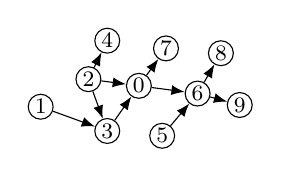
\begin{tikzpicture}[font={\footnotesize}, every node/.style={draw, inner sep=0 pt, minimum size=9 pt,
circle, fill=white}]
[font=\footnotesize, label distance=0 cm, inner sep=0.5 pt,
every node/.style={anchor=center},
]

\path
(0,0) node (a1) {\(1\)}
-- ++(30:0.7) node (a2) {\(2\)}
-- ++(-70:0.7) node (a3) {\(3\)}
-- ++(55:0.7) node (a0) {\(0\)}
-- ++(125:0.7) node (a4) {\(4\)}
(a3) ++(-5:0.7) node (a5) {\(5\)}
-- ++(50:0.7) node (a6) {\(6\)}
-- ++(125:0.7) node (a7) {\(7\)}
-- ++(-05:0.7) node (a8) {\(8\)}
-- ++(-70:0.7) node (a9) {\(9\)}
;

% site dependencies
\begin{scope}[-Latex]

\draw (a0) -- (a6) ;
\draw (a0) -- (a7) ;
\draw (a1) -- (a3);
\draw (a2) -- (a0) ;
\draw (a2) -- (a3) ;
\draw (a2) -- (a4) ;
\draw (a3) -- (a0) ;
\draw (a5) -- (a6) ;
\draw (a6) -- (a8) ;
\draw (a6) -- (a9) ;

\end{scope}

\end{tikzpicture}
\end{document}
